\section{Evaluation of PREF for traffic splitting}

An individual evaluation of PREF, the splitting mechanism of PREFLEX, is required to understand better the global performance of PREFLEX. Indeed, the two components PREF and LEX are functionally separate. Hence, in this section PREF will be disassociated from the rest of the architecture and put in two other contexts. A simplified load balancer, referred to in this text as “equalization mode”, that balances the traffic in a fixed and equal fraction over all the available paths. The second scenario, is in a simplified version of TEXCP that doesn't include the core routers based traffic shaping for congestion management. 

For both modes, we are going to use the topology ..,. The variation of the number pf flows in the system is kept simple with the same number of flows for both servers. Only one change was introduced to see how fast is the reaction of the algorithm. It concerns the number of flows for each destination.

\subsection{Equalization Mode}

In this mode each balancer defines an equal split over the three paths for each of the destination. Figure \ref{fig:fwnd} gives an example

 \begin{figure}[h]
  \begin{center}
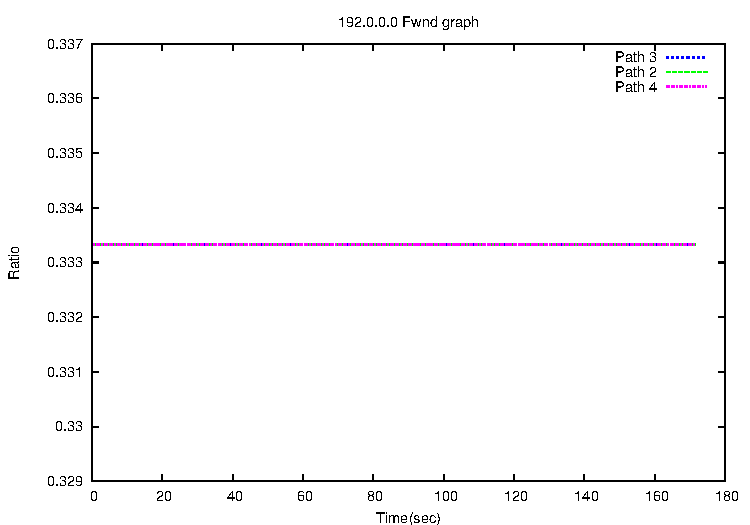
\epsfig{file=img/results/fwnd-192-0-0-0, width=4.5in}
\caption{
  Flowlet ratio $f_{i}$ for destination $E_{1}$ as set by ingress point $I_{1}$.
    \label{fig:fwnd}
}
 \end{center}
\end{figure}

The graphs bellow show the throughput of the traffic that ingress node I1 send over each link.\\

PREF

\begin{figure}[h]
 \begin{center}

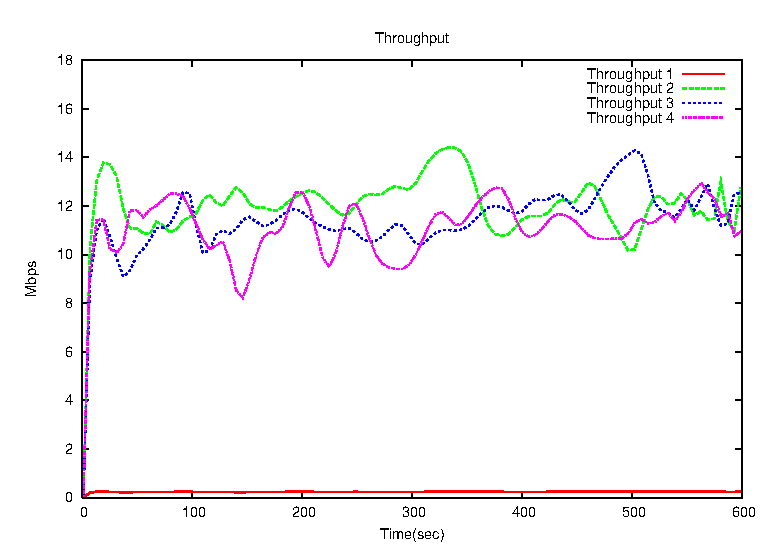
\epsfig{file=img/results/sec5-1/equalization-PREF/eleven/throuputs, width=4.5in}
\caption{
  Throughputs over each interface.
    \label{fig:equal-thro-pref}
}
\end{center}

FLARE

\end{figure}

 \begin{figure}[h!]
 \begin{center}
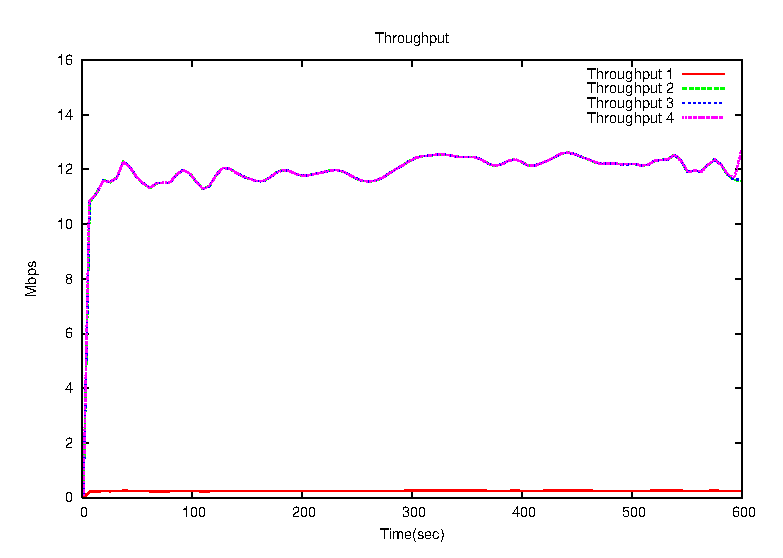
\epsfig{file=img/results/sec5-1/equalization-FLARE/eleven/throuputs, width=4.5in}
\caption{
  Throughputs over each interface.
    \label{fig:equal-thro-flare}
}
\end{center}

\end{figure}

%\begin{figure}[h]
%  \begin{center}
%    \mbox{
%      \subfigure[]{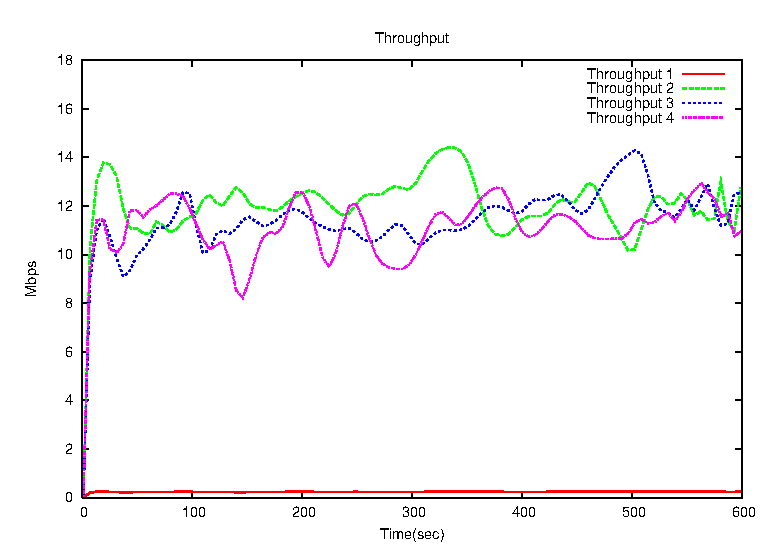
\includegraphics[width=4.0in]{img/results/sec5-1/equalization-PREF/eleven/throuputs}}\\
%      \subfigure[]{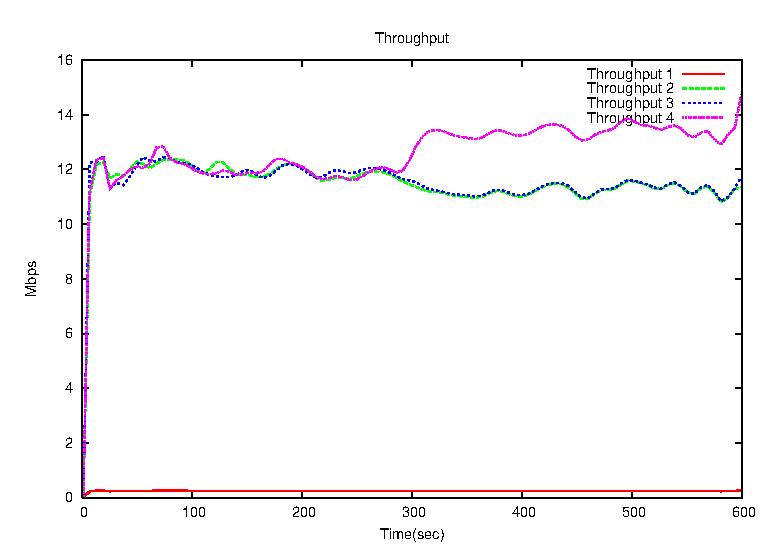
\includegraphics[width=4.0in]{file=img/results/sec5-1/equalization-FLARE/eleven/throuputs}}
%    }
%\caption{caption goes here.}
%\label{fig:parts}
%\end{center}
%\end{figure}

As expected, PREF which is equibalen a flow based traffic splitor, doesn't match the accuracy level of FLARE in splitting the traffic, but still the difference on the throughput over each path stays limited. The graphs also show oscillation behaviour of PREF. We find the same oscillation behaviour in the graphs of drop rate at the bottlenecks.

PREF

\begin{figure}[h]
 \begin{center}

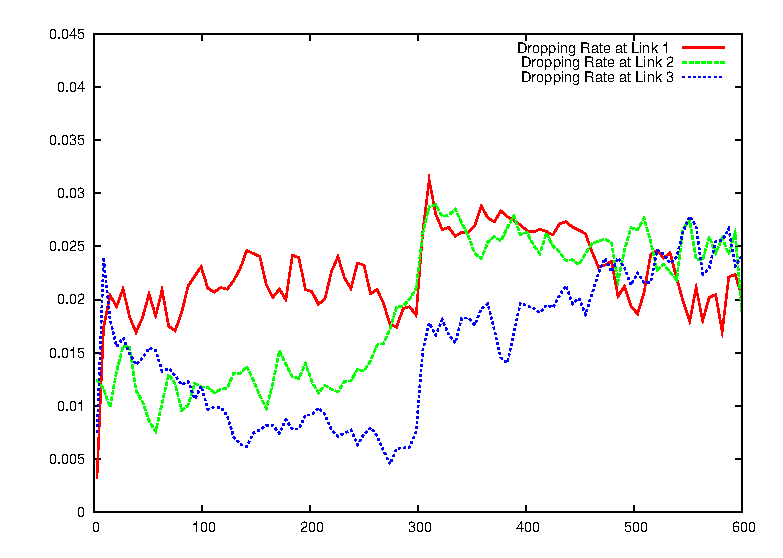
\epsfig{file=img/results/sec5-1/equalization-PREF/dropRate, width=4.5in}
\caption{
  Drop Rate at the botlenecks.
    \label{fig:equal-thro-pref}
}
\end{center}
\end{figure}

FLARE
 \begin{figure}[h!]
 \begin{center}
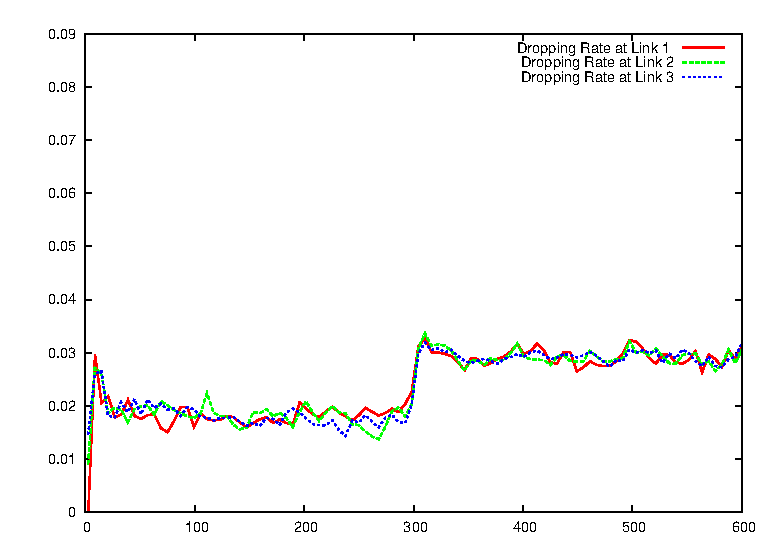
\epsfig{file=img/results/sec5-1/equalization-FLARE/dropRate, width=4.5in}
\caption{
  Drop Rate at the botlenecks.
    \label{fig:equal-thro-flare}
}
\end{center}
\end{figure}

These seconds graphs provide a hint about the reason of the fluctuation. The path assignement process of PREF makes the flowlets, which are transport aware, evolve their whole life cycle in one path and hence have a different congestion experience than the other flows. As a result, their tranmission rates and the congestion that they are making ares decorrelated.In the other hand, the network flowlets used by FLARE are a smaller order of granuilarity and makes that the transport flows get a path attributed multiple times during their flow time. As a result, the congestion level that a TCP routine experienced is a combination of the congestion in the different paths and hence the flows adapt their tranmission rate to a common level of congestion and the fluctuations are less significant.

%\clearpage

\subsection{balancing by path utilization}

Now we consider the example of balancing by path utilization, a simplified version of TEXCP where ingress points don't use the core routers feedback to control their transmissions rate.

PREF

\begin{figure}[h]
 \begin{center}

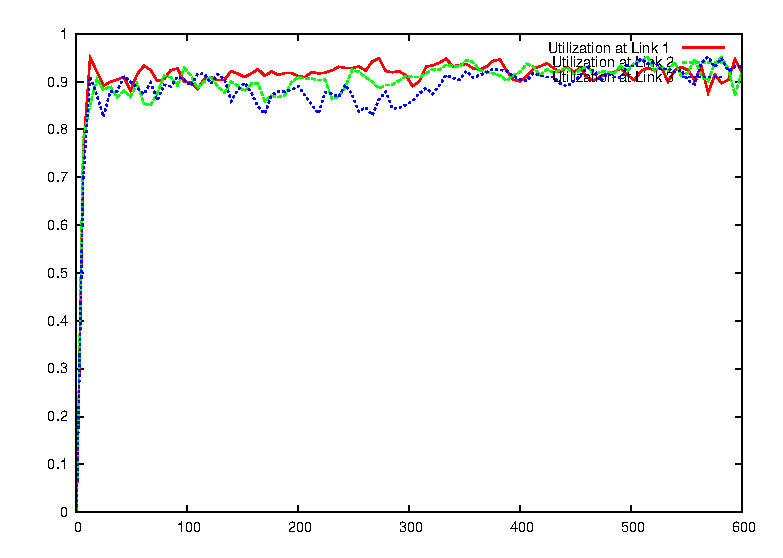
\epsfig{file=img/results/sec5-1/equalization-PREF/util, width=4.5in}
\caption{
  Path utilization measured at bottlenecks. 
    \label{fig:texcp-util-pref}
}
\end{center}
\end{figure}

FLARE
 \begin{figure}[h!]
 \begin{center}
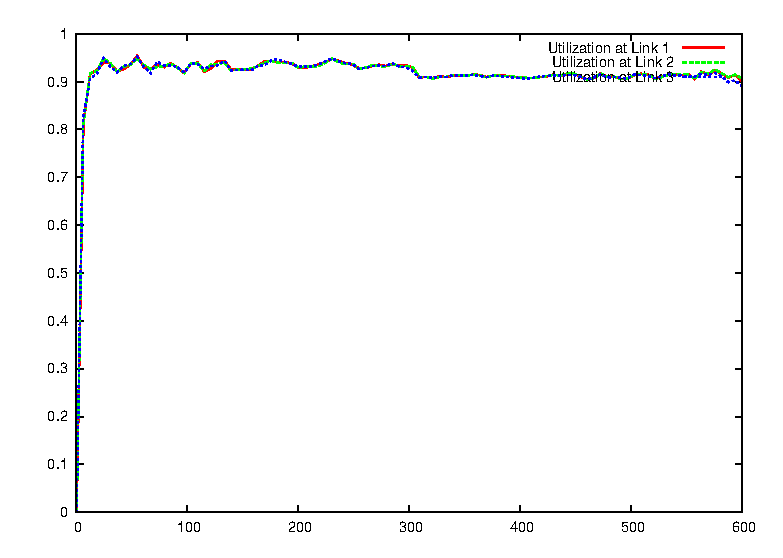
\epsfig{file=img/results/sec5-1/texcp-flare/util, width=4.5in}
\caption{
  Path utilization measured at bottlenecks. 
    \label{fig:texcp-util-flare}
}
\end{center}
\end{figure}

The previous analysis is stil valid ine the case of balamcing by path utilization. This last parameter oscillates in the case of PREF splitting, and equalization is not achieved with the same accuracy.

\paragraph{Conclusion}

Splitting traffic using PREF is required for the congestion mechanism defined by LEX. The revelation of a path congestion requires that the retranmitted packets follow the same path. Moreover, it makes congestion bakancing a bit more difficult since the flows follow one path with decorelated congestion experiences. However, PREF allows path diversity schemes at end hosts and network to coexist. The performance of PREF could be enhanced further, if efficient strategies of how and when to trigger path selection were deployed at by the recievers.
 
%\section{Load balancing VS congestion balancing}
\section{Analysis of PREFLEX balancing algorithm}

In this section we are going to evaluate the performance of the algorithm for different configuration parameters. 

\subsection{Decision time interval}

The decision time interval is an external parameter for the algorithm. It determines how often the network domain call to update the split. The raction of the algorithm and how long it takes to reach equilibrium is linked to the decision interval. But from another hand, this decision interval is also dependant of the period over which the loss signals are aggregated. As a result, a frequent update of the split may result in a unstability of the system that will be even stressed when the aggregation time of the losses is carried out for small periods of time. In practice, we choose the decision time interval to the double of the time value for the aggregation.

The graphs bellow show the dropping rate observed at the bottleneck. 

\begin{figure}[h]
 \begin{center}

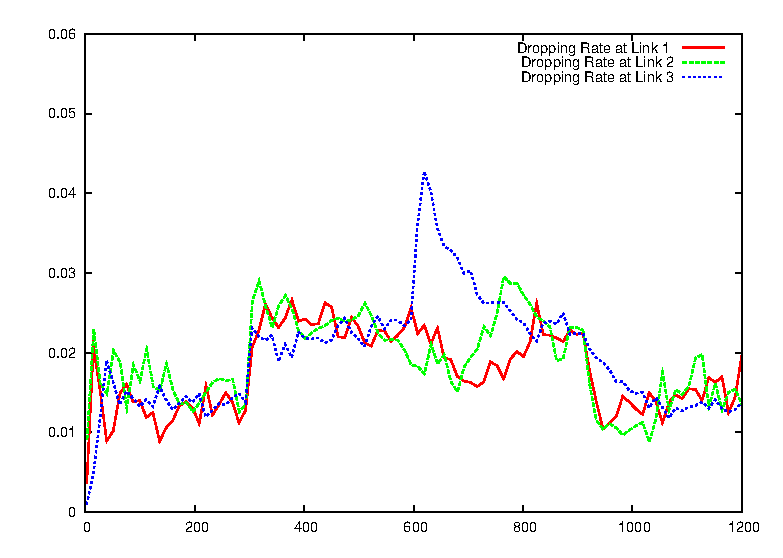
\epsfig{file=img/sec-5-2-1/eight/dropRate, width=4.5in}
\caption{
  Drop Rate at the botlenecks. 
    \label{fig:split-eight}
}
\end{center}
\end{figure}

%FLARE
 \begin{figure}[h!]
 \begin{center}
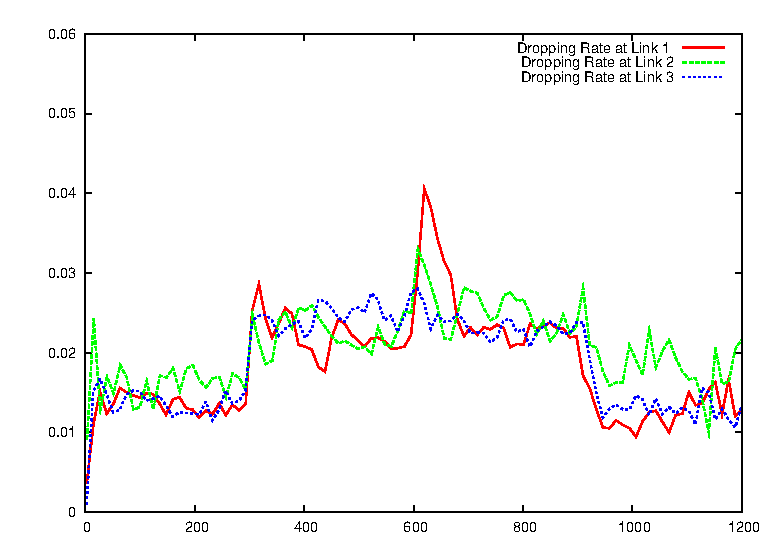
\epsfig{file=img/sec-5-2-1/four/dropRate, width=4.5in}
\caption{
  Drop Rate at the botlenecks.
    \label{fig:split-time-four}
}
\end{center}
\end{figure}

\clearpage

{\bf Update interval: 1sec}

\begin{figure}[h]
 \begin{center}

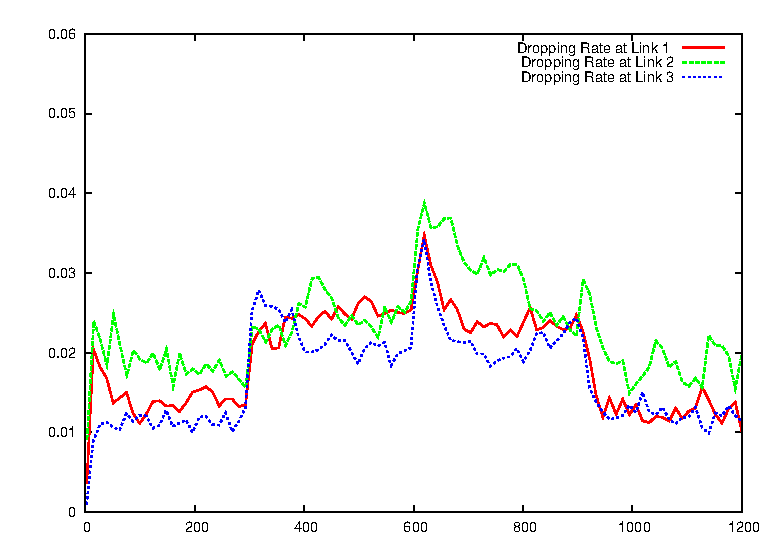
\epsfig{file=img/sec-5-2-1/one/dropRate, width=4.5in}
\caption{
  Drop Rate at the botlenecks.
    \label{fig:split-one}
}
\end{center}
\end{figure}

As expected, whith a small update interval the algorithm acts more aggresively and doesn't leave enough time for the flows to reach stability. As a result the congestion level experienced in the different paths (expressed by the dropping rate at each bottleneck) is not well balanced. A larger time intervals (8 and 4 sec) allow to achieve a better balancing of the congestion over the available paths and with an enhanced stability. From the different simulations that we've carried out, an update interval between 40 to 100 RTT (apprixmately 100ms for the simulations here) allowed to achieve most of the time a good accuracy of the congestion balancing. An even higher value for the update interval turns the balancer too slow. This effect could be illustrated with the reaction of the system for sudden and important change in traffic demand. We could see at around the second 600, when the demand on traffic turned from a destination to another one, the balancer with an update interval of 4 sec required slightly less time to achieve equiblruim.    
 
 \clearpage

%\begin{figure}[htbp]
%\begin{center}
%\subfloat[]{
%\label{rcpstart4}
%\includegraphics[scale=0.4]{plots/lan/1.5Mb/rcp/flowstart4.eps}}
%\hspace{10mm}
%\subfloat[]{
%\label{xcprcpstart4}
%\includegraphics[scale=0.4]{plots/lan/1.5Mb/xcp0/flowstart4.eps}}
%\caption{The throughput of end-hosts and the router queue as a fourth flow starts, using \protect\subref{rcpstart4} RCP and \protect\subref{xcprcpstart4} XCP.}
%\label{rcpstart4comp}
%\end{center}
%\end{figure}

\subsection{PREFLEX balancing modes}

In this section we are going to analye PREFLEX balancing mode: Equalizatiom, Conservative and Loss Driven.

Reminder
$\beta_{E}$, $\beta_{C}$ and $\beta_{L}$ denotes positive factors associated consecutively with “equalization” $E$, “conservative” $C$, and “loss driven” $L$ modes.

{\bf Conservative mode} : $\beta_{E}=0$, $\beta_{C}=1$ and $\beta_{L}=0$
\\The conservative mode doesn't achieve an acurate congestion balancing over the available paths. But more importantly, the split as defined by this mode is not stable. Though it can't be used to stabilize the performance of the balancer. A plausible explanation is limitation of the assumption that the flow fraction is equalt to byte fraction, when the loss rates of paths aren't equivalent.

\begin{figure}[h!]
 \begin{center}

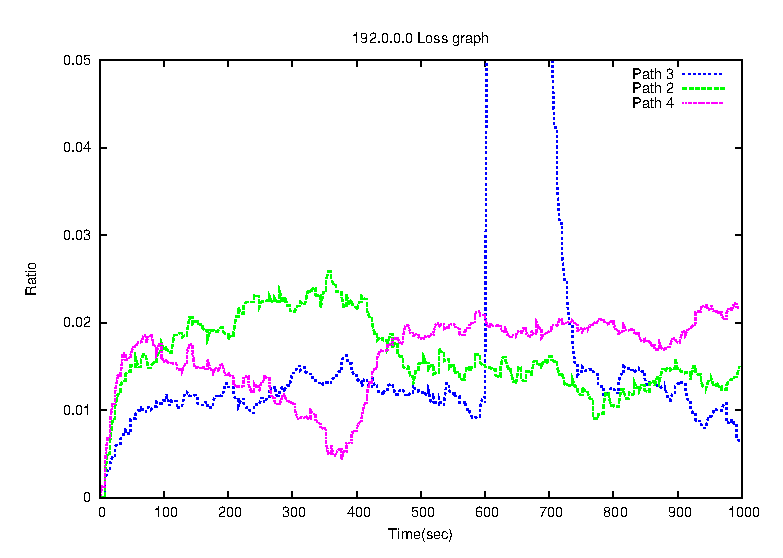
\epsfig{file=img/sec-5-2-2/Alt-split-0-100-0/loss-192-0-0-0, width=4.5in}
\caption{
   Loss ratio $\rho_{i}$ for destination E1 as seen by balancer P in consrvative mode.

    \label{fig:splitCon-loss}
}
\end{center}
\end{figure}

\clearpage
\begin{figure}[h!]
 \begin{center}

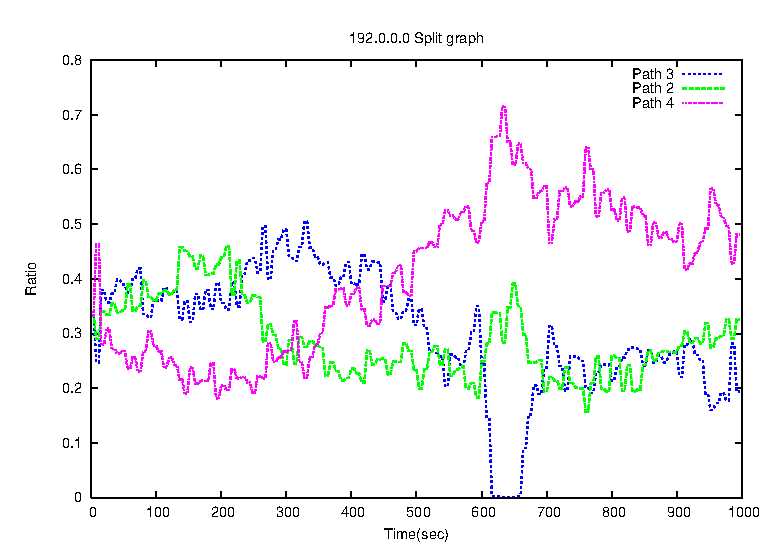
\epsfig{file=img/sec-5-2-2/Alt-split-0-100-0/fwnd-192-0-0-0, width=4.5in}
\caption{
   The desired split that balancer P set for destination E1 in conservative mode.

    \label{fig:splitCon-fwnd}
}
\end{center}
\end{figure}


{\bf Equalization} : $\beta_{E}=1$, $\beta_{C}=0$ and $\beta_{L}=0$
\\As depicted by figure \ref{fig:splitEqual-loss}, an equal distribution of flows over the paths doesn't achieve an equal balancing of loss. Moreover, its performance depends on the traffic nature in the network. Path 3 underutilized illustrates the suboptimal nature of equal balancing. Also the difference of congestion levels in the other two paths is directly linked to changes in traffic demand. During the change on traffic demand between time 200sec and 600sec, the difference between the congestion levels sigificantly increased.

However, the real contribution of the "equal" mode is to ensure that a minimum number of flows are sent over each path. In fact, as we are going to see next, the accuracy of the loss estimation made by the loss balancer depends on the number of flows sent over the path. 

\clearpage
\begin{figure}[h]
 \begin{center}

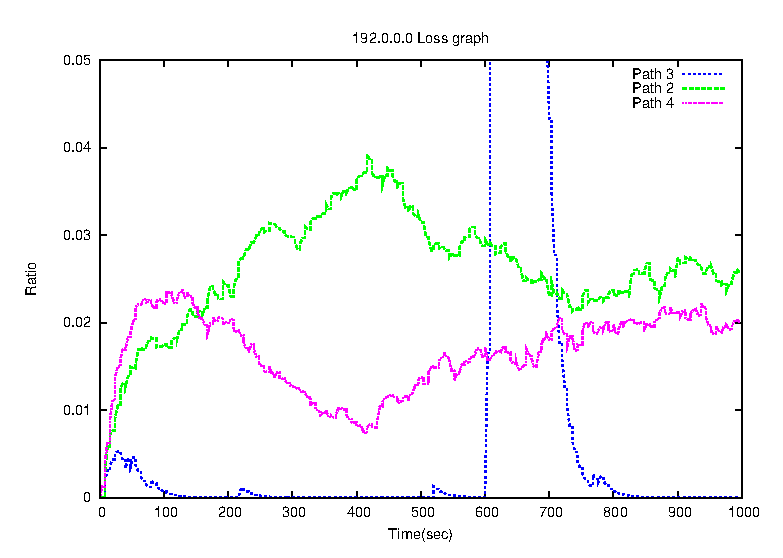
\epsfig{file=img/sec-5-2-2/Alt-split-0-0-100/loss-192-0-0-0, width=4.5in}
\caption{
   Loss ratio $\rho_{i}$ for destination E1 as seen by balancer P in equalisation mode.

    \label{fig:splitEqual-loss}
}
\end{center}
\end{figure}


{\bf Unbounded loss driven mode} : $\beta_{E}=0$, $\beta_{C}=0$ and $\beta_{L}=1$
\\Figures \ref{fig:splitpureLoss-fwnd1} and \ref{fig:splitpureLoss-fwnd1} show that the balancer allocate different splits for destination E1 and E2 even when the system is symetric for the two destination. This is explained by the fact that balancing for the two destination is carried seperately which is natural since the flows for the two destinations. This is natural since the paths for the two destination are different even if they share the same bottleneck in our topology. But there is no one optimal split, and the balancer suceeds though during the first 200 sec in balance the congestion equally for both destination (see \ref{fig:splitpureLoss-loss1} and \ref{fig:splitpureLoss-loss2}). But by keeping to send less E2 flows on the path, the accuracy of the loss estimation become low and different from E1 flows. In particular, it is over estimated what accelerate more the drop. As a result the equalization mode is used to make sure that there are enough flows on every pathfor an accurate estimation of the loss.

\begin{figure}[h]
 \begin{center}

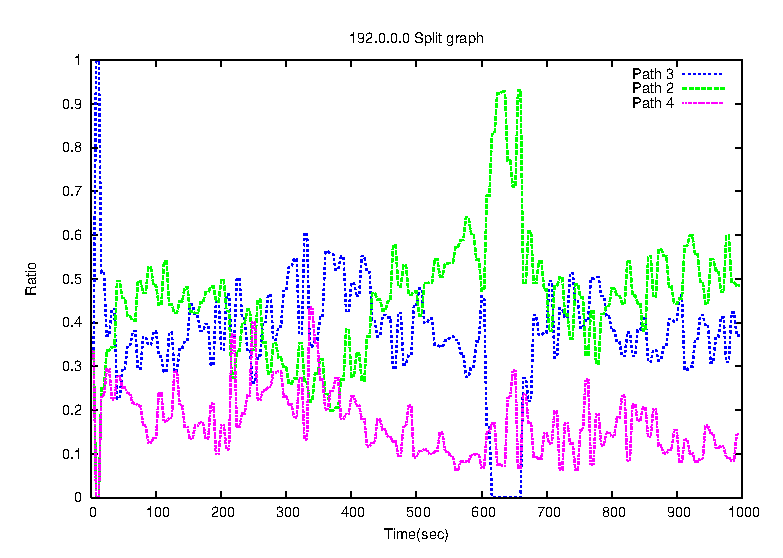
\epsfig{file=img/sec-5-2-2/Alt-split-100-0-0/fwnd-192-0-0-0, width=4.5in}
\caption{
   The desired split that balancer P set for destination E1 in unbounded loss driven mode.

    \label{fig:splitpureLoss-fwnd1}
}
\end{center}
\end{figure}

\begin{figure}[h]
 \begin{center}

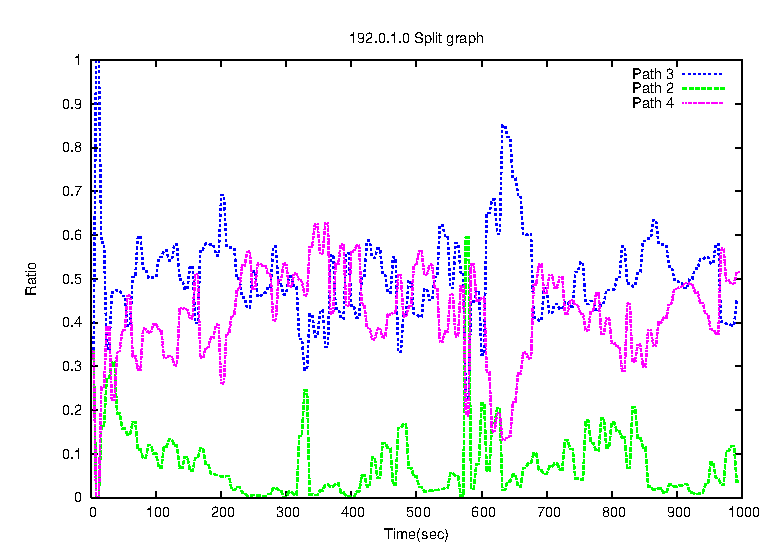
\epsfig{file=img/sec-5-2-2/Alt-split-100-0-0/fwnd-192-0-1-0, width=4.5in}
\caption{
   The desired split that balancer P set for destination E2 in unbounded loss driven mode.

    \label{fig:splitpureLoss-fwnd2}
}
\end{center}
\end{figure}


\begin{figure}[h]
 \begin{center}

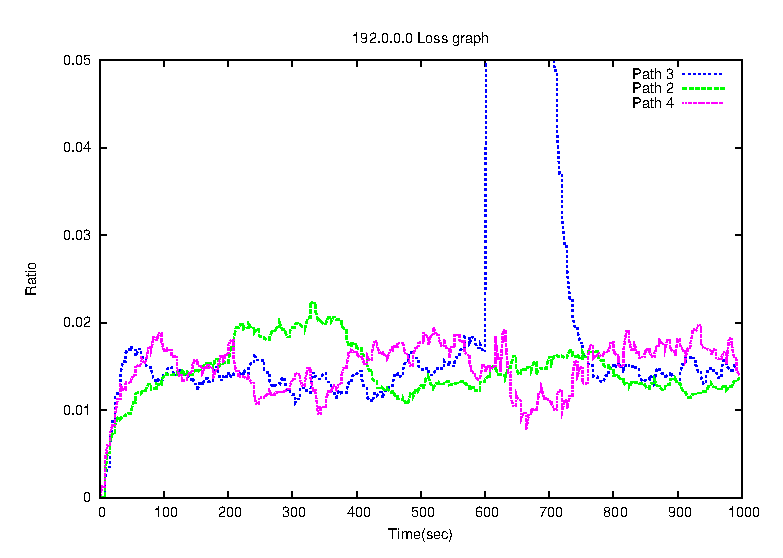
\epsfig{file=img/sec-5-2-2/Alt-split-100-0-0/loss-192-0-0-0, width=4.5in}
\caption{
   Loss ratio $\rho_{i}$ for destination E1 as seen by balancer P in unbounded loss driven mode.

    \label{fig:splitpureLoss-loss1}
}
\end{center}
\end{figure}

\begin{figure}[h]
 \begin{center}

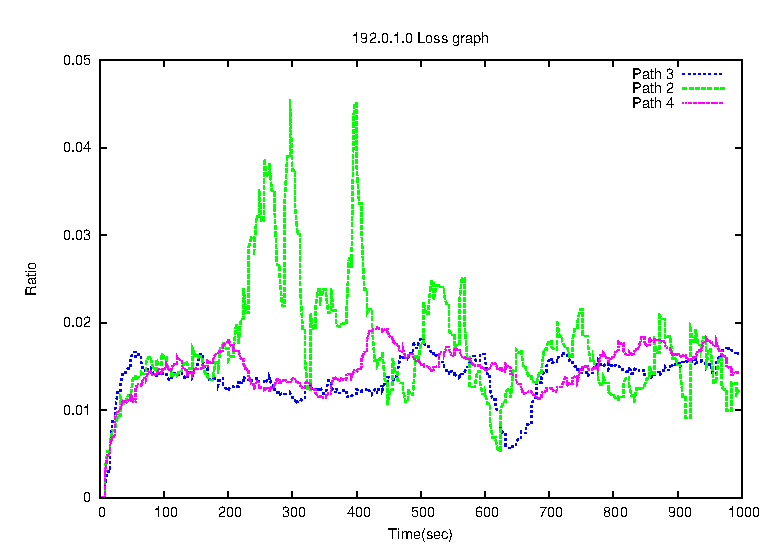
\epsfig{file=img/sec-5-2-2/Alt-split-100-0-0/loss-192-0-1-0, width=4.5in}
\caption{
   Loss ratio $\rho_{i}$ for destination E2 as seen by balancer P in unbounded loss driven mode.

    \label{fig:splitpureLoss-loss2}
}
\end{center}
\end{figure}

\clearpage

{\bf Bounded loss driven mode} : $\beta_{E}=0.9$, $\beta_{C}=0$ and $\beta_{L}=0.1$
\\By allocating a share of the traffic to be equally distributed we guarantee that a minmum number of flows is sent over each path to continue probing the path in question and accurately estimate its level of congestion. The effect of this boundary is clearly shown in the loss distribution compared to the previous mode \ref{fig:splitlossD-loss1} and \ref{fig:splitlossD-loss2}. Though, the  booked share for equalization should be too high to block the loss equalization process. 

In another hand, \ref{fig:splitlossD-fwnd1} and \ref{fig:splitlossD-fwnd1} {\bf Something about failure}


\begin{figure}[h]
 \begin{center}

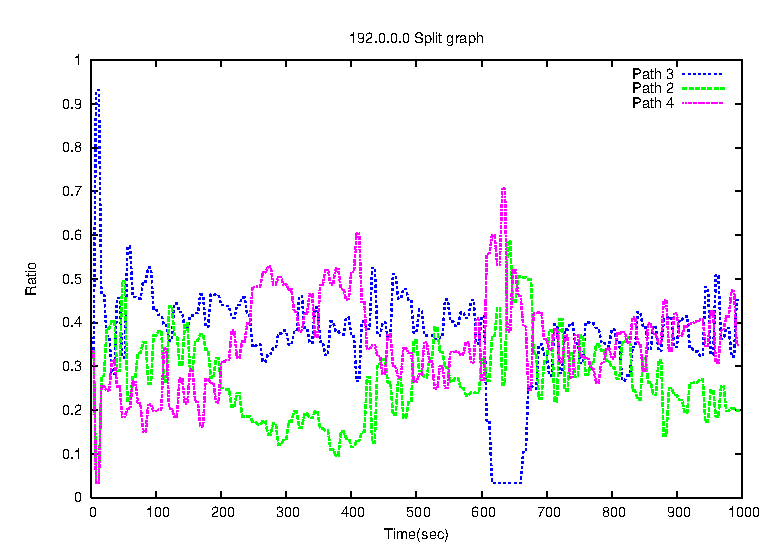
\epsfig{file=img/sec-5-2-2/Alt-split-90-0-10/fwnd-192-0-0-0, width=4.5in}
\caption{
   The desired split that balancer P set for destination E1 in "pure" loss driven mode.

    \label{fig:splitlossD-fwnd1}
}
\end{center}
\end{figure}

\begin{figure}[h]
 \begin{center}

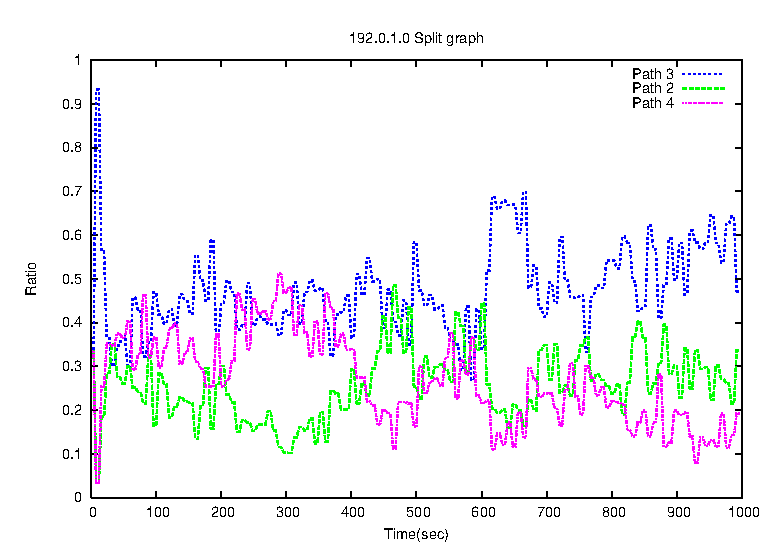
\epsfig{file=img/sec-5-2-2/Alt-split-90-0-10/fwnd-192-0-1-0, width=4.5in}
\caption{
   The desired split that balancer P set for destination E2 in "pure" loss driven mode.

    \label{fig:splitlossD-fwnd2}
}
\end{center}
\end{figure}


\begin{figure}[h]
 \begin{center}

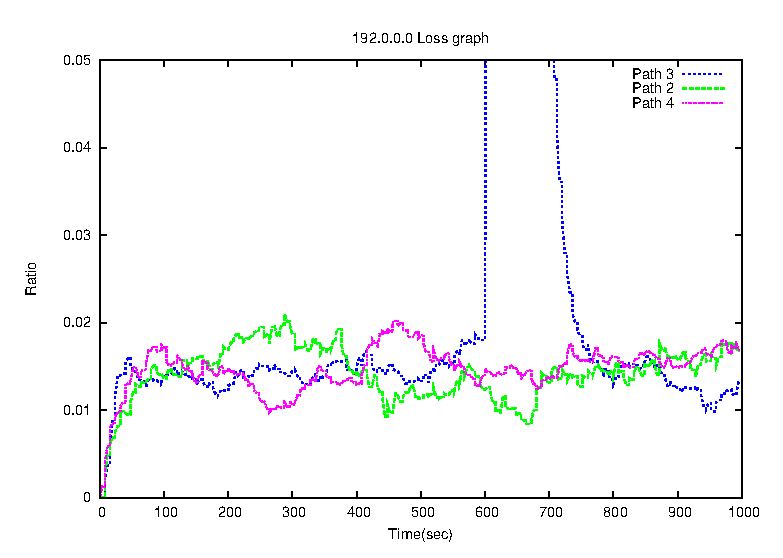
\epsfig{file=img/sec-5-2-2/Alt-split-90-0-10/loss-192-0-0-0, width=4.5in}
\caption{
   Loss ratio $\rho_{i}$ for destination E1 as seen by balancer P in "pure" loss driven mode.

    \label{fig:splitlossD-loss1}
}
\end{center}
\end{figure}

\begin{figure}[h]
 \begin{center}

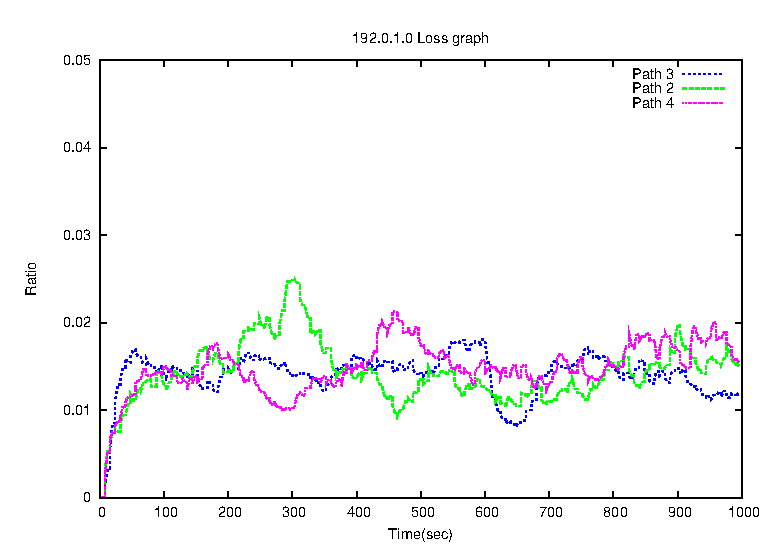
\epsfig{file=img/sec-5-2-2/Alt-split-90-0-10/loss-192-0-1-0, width=4.5in}
\caption{
   Loss ratio $\rho_{i}$ for destination E2 as seen by balancer P in "pure" loss driven mode.

    \label{fig:splitlossD-loss2}
}
\end{center}
\end{figure}

\clearpage

\section{Comparison between PREFLEX and TEXCP}

\subsection{Balancing by path utilization}
